\documentclass[border=5pt]{standalone}
\usepackage{fontspec,unicode-math}
\setmainfont{Noto Serif}
\setmathfont{STIXTwoMath-Regular.otf}
\usepackage{tikz}
\usetikzlibrary{arrows.meta,calc,patterns,decorations.markings,decorations.pathmorphing}
\tikzset{lev/.style={line width=1.25pt,line cap=butt},
 fine/.style={line width=.60pt},band/.style={line width=.57pt},
 curve/.style={line width=1.35pt,line cap=round,line join=round},
 ax/.style={line width=.65pt,-{Latex[length=2.3mm,width=1.3mm]}},
 ray/.style={line width=.68pt,-{Latex[length=2.0mm,width=1.10mm]}},
 dimension/.style={line width=.57pt,{Latex[length=1.7mm,width=.9mm]}-{Latex[length=1.7mm,width=.9mm]}},
 flow/.style={line width=.68pt,postaction={decorate},decoration={markings,mark=at position .66 with {\arrow{Latex[length=2mm,width=1.1mm]}}}},
 lab/.style={font=\fontsize{13}{16}\selectfont,inner sep=1.3pt},
 small/.style={font=\fontsize{11}{13}\selectfont,inner sep=1.2pt},
 tinytext/.style={font=\fontsize{10}{12}\selectfont,inner sep=1pt},
 panel/.style={font=\fontsize{14}{16}\selectfont\itshape,inner sep=0pt}}
\pagestyle{empty}
\begin{document}
% CP14: k-indexed Floquet replicas, descending by one hbar omega_2 per step.
% This display is schematic; n* values are level labels, not measured energy coordinates.
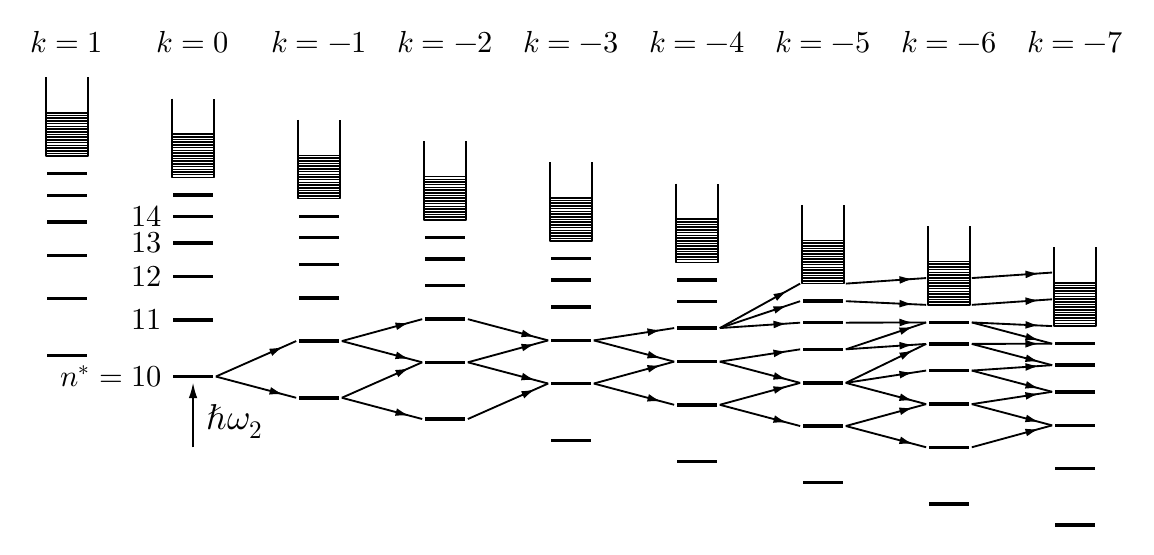
\begin{tikzpicture}[x=1cm,y=1cm,line join=round]
\tikzset{flow/.style={line width=.67pt,postaction={decorate},
 decoration={markings,mark=at position .84 with {\arrow{Latex[length=1.75mm,width=1mm]}}}}}
% Each replica has six explicit Rydberg levels and a 17-line quasicontinuum.
\foreach \col/\idx in {0/1,1/0,2/-1,3/-2,4/-3,5/-4,6/-5,7/-6,8/-7}{
 \pgfmathsetmacro{\cxx}{.8+1.6*\col}
 \pgfmathsetmacro{\yybase}{1.2697-.26975*\col}
 \node[small] at (\cxx,5.25) {$k=\idx$};
 \foreach \drop in {0,.72025,1.26805,1.69438,2.03265,2.3056}{
   \draw[lev] (\cxx-.25,\yybase+\drop)--++(.50,0);}
 \foreach \q in {0,...,16}{
   \draw[band] (\cxx-.27,\yybase+2.5289+.034375*\q)--++(.54,0);}
 \draw[fine] (\cxx-.27,\yybase+3.5289)--(\cxx-.27,\yybase+2.5289)
     --(\cxx+.27,\yybase+2.5289)--(\cxx+.27,\yybase+3.5289);
}
% Author's n* enumeration at k=0. The unlabeled highest discrete level is preserved.
\foreach \lab/\yy in {10/1.0000,11/1.72025,12/2.26805,13/2.69438,14/3.03265}{
 \node[small,anchor=east,fill=white,inner sep=1pt] at (2.045,\yy) {$\ifnum\lab=10 n^*=\fi\lab$};}
% Every transition retains its CP13 endpoint and index direction k -> k-1.
\draw[flow] (2.69000,1.00000)--(3.71000,0.73025);
\draw[flow] (2.69000,1.00000)--(3.71000,1.45050);
\draw[flow] (4.29000,1.45050)--(5.31000,1.18075);
\draw[flow] (4.29000,1.45050)--(5.31000,1.72856);
\draw[flow] (4.29000,0.73025)--(5.31000,0.46050);
\draw[flow] (4.29000,0.73025)--(5.31000,1.18075);
\draw[flow] (5.89000,1.72856)--(6.91000,1.45881);
\draw[flow] (5.89000,1.18075)--(6.91000,0.91100);
\draw[flow] (5.89000,1.18075)--(6.91000,1.45881);
\draw[flow] (5.89000,0.46050)--(6.91000,0.91100);
\draw[flow] (7.49000,1.45881)--(8.51000,1.18906);
\draw[flow] (7.49000,1.45881)--(8.51000,1.61538);
\draw[flow] (7.49000,0.91100)--(8.51000,0.64125);
\draw[flow] (7.49000,0.91100)--(8.51000,1.18906);
\draw[flow] (9.09000,1.61538)--(10.11000,1.68390);
\draw[flow] (9.09000,1.61538)--(10.11000,1.95681);
\draw[flow] (9.09000,1.61538)--(10.11000,2.18016);
\draw[flow] (9.09000,1.18906)--(10.11000,0.91931);
\draw[flow] (9.09000,1.18906)--(10.11000,1.34563);
\draw[flow] (9.09000,0.64125)--(10.11000,0.37150);
\draw[flow] (9.09000,0.64125)--(10.11000,0.91931);
\draw[flow] (10.69000,2.18016)--(11.71000,2.25064);
\draw[flow] (10.69000,1.95681)--(11.71000,1.91041);
\draw[flow] (10.69000,1.68390)--(11.71000,1.68706);
\draw[flow] (10.69000,1.34563)--(11.71000,1.41415);
\draw[flow] (10.69000,1.34563)--(11.71000,1.68706);
\draw[flow] (10.69000,0.91931)--(11.71000,0.64956);
\draw[flow] (10.69000,0.91931)--(11.71000,1.07588);
\draw[flow] (10.69000,0.91931)--(11.71000,1.41415);
\draw[flow] (10.69000,0.37150)--(11.71000,0.10175);
\draw[flow] (10.69000,0.37150)--(11.71000,0.64956);
\draw[flow] (12.29000,2.25064)--(13.31000,2.32071);
\draw[flow] (12.29000,1.91041)--(13.31000,1.98089);
\draw[flow] (12.29000,1.68706)--(13.31000,1.41731);
\draw[flow] (12.29000,1.68706)--(13.31000,1.64066);
\draw[flow] (12.29000,1.41415)--(13.31000,1.14440);
\draw[flow] (12.29000,1.41415)--(13.31000,1.41731);
\draw[flow] (12.29000,1.07588)--(13.31000,0.80613);
\draw[flow] (12.29000,1.07588)--(13.31000,1.14440);
\draw[flow] (12.29000,0.64956)--(13.31000,0.37981);
\draw[flow] (12.29000,0.64956)--(13.31000,0.80613);
\draw[flow] (12.29000,0.10175)--(13.31000,0.37981);
% Photon-energy arrow is tied to initial level n*=10, not an arbitrary text offset.
\draw[ray] (2.40,.100)--(2.40,.925);
\node[lab,anchor=west] at (2.52,.43) {$\hbar\omega_2$};
\end{tikzpicture}
\end{document}
